\chapter{Experiments} \label{experiments_chapter}

In previous chapters I have presented the dataset (chapter \ref{chapter:data}), and discussed challenges which arise from its properties (chapter \ref{chapPreproc}). Next I described the neural network architectures (chapter \ref{neural_nets_chapter}) which served as building blocks for the models introduced in chapter \ref{model_chapter}. Now I want to connect all the parts together, elaborate on the trainining of the models (e.g. used optimizer, calculated metrics, hyperparameter choice) and analyze their results.

Let me recap the main challenges we face, and hypothesize about the ideal generation system. Firstly, the target summaries are really long. The ideal system should remember what has already been generated and shouldn't produce duplications. Secondly, the targets contain a lot of facts based on the input structured data. The ideal system should copy these facts from the input and reduce \emph{hallucinations}. Lastly, the generated text should be as close to English as possible \emph{while meeting the requirements described previously}.

\section{Development Methods}

The proposed models solve the task in \emph{end-to-end} manner. Given an input table $\boldsymbol{x}$ and the corresponding gold output summary $\boldsymbol{y}$ the model approximates the conditional probability of the latter conditioned on the former $p(\boldsymbol{y} | \boldsymbol{x})$. Following the maximum likelihood principle (e.g. section 5.5 in \citep{Goodfellow-et-al-2016}) the models are trained to minimize the cross-entropy loss (negative log likelihood) on the training set $\mathcal{D}$.(equation \ref{equation:negative_log_likelihood}).

\begin{equation} \label{equation:negative_log_likelihood}
    - \sum_{(\boldsymbol{x}, \boldsymbol{y}) \in \mathcal{D}}{log\ p_{model}(\boldsymbol{y} | \boldsymbol{x})}
\end{equation}

As explained in section \ref{subsection:high_level_encoder_decoder} the training happens under \emph{teacher-forcing} setting. The minimization is provided by stochastic gradient descent, specifically we opted to use one of the standard algorithms, Adam \citep{kingma2014adam}. Since this algorithm associates specific learning rate to each of the trainable network parameters, we modify only the initial learning rate parameter\footnote{It means that we don't try e.g. learning rate decay.}.

We report the loss value as well as the accuracy of the model (the frequency with which the most probable token in the distribution generated by the model matches the gold token), to be able to detect \emph{underfitting} (this happens when a model is unable to obtain sufficiently low loss value on the training set).

However we are not interested in the performance of the model on the training set. The main challenge is to create a model which will be able to perform well on previously unseen data. Therefore we report the loss value, and the accuracy of the model on the development part of the dataset (also collected under \emph{teacher-forcing} setting). We consider the model with the lowest loss value and accuracy on the development set to be the best.

\section{Generation}

As explained in section \ref{subsection:high_level_encoder_decoder}, during inference we want to find a sequence of tokens $y_1,\dots,y_n$ which maximizes the probability
\begin{equation}
    p_{model}(\boldsymbol{y} | \boldsymbol{x}) = \prod_{t=1}^N{p_{model}(y_t|y_1,\dots,y_{t-1}, \boldsymbol{x})}
\end{equation}

Since it is computationally  unfeasible to compute the probabilities of all the output sequences and to choose the best one we only approximate the optimal sequence.

\subsection{Greedy Decoding}

Greedy Decoding provides the simplest approximation of the optimal sequence. At each time-step we take the most probable token under the model distribution as the output. The process ends when the \emph{\textless EOS\textgreater} token is generated.
\begin{align*}
    \hat{y}_1 &= \argmax_{y'}{p_{model}(y' | \boldsymbol{x})} \\
    \hat{y}_2 &= \argmax_{y'}{p_{model}(y' | \hat{y}_1, \boldsymbol{x})} \\
    &\dots \\
    <EOS> &= \argmax_{y'}{p_{model}(y' | \hat{y}_1,\dots,\hat{y}_{n'}, \boldsymbol{x})}
\end{align*}

The suboptimality of the algorithm can be seen on a simple example. E.g. let's say that we have a training corpus consisting of sentences describing my eating habits. The corpus consists of sentences "I eat a banana", "I eat a peach", "I eat a goulash" and two repetitions of sentence "I eat an apple". Starting from the state after generating subsequence "I eat", the greedy decoder would pick "a" as the most probable continuation of the sequence. However the optimal solution would have picked "an", because none of the possible continuations of subsequence "I eat a" is as probable as "I eat an apple" which is the most occuring sentence in the corpus.

\subsection{Beam Search Decoding}

Beam Search builds on the greedy decoding approach. We keep track of $k$ most promising \emph{hypotheses} (and associated hidden states). A hypothesis is a sequence of generated tokens $y_1,\dots,y_{n'}$. We compute its score (equation \ref{equation:hypothesis_score}).
\begin{equation} \label{equation:hypothesis_score}
    score(y_1,\dots,y_{n'}) = \sum_{i=1}^{n'}{\log{p(y_i | y_1, \dots, y_{i-1}, \boldsymbol{x})}}
\end{equation}

At each time-step we expand all the hypotheses (take $k$ most probable tokens under the respective hypothesis, which will result in $k^2$ possibilities), and choose $k$ with the highest score. $k$ is called the \emph{beam size}. An example of the approach can be seen in figure \ref{figure:beam_search}.

\begin{figure}[!h]
    \centering
    \includegraphics[scale=0.2]{img/beam_search.png}
    \caption{\centering Beam-Search decoding, excerpt from the slides to lecture about Machine Translation, Seq2Seq and Attention on Stanford \url{http://web.stanford.edu/class/cs224n/}} \label{figure:beam_search}
\end{figure}

\section{Evaluation Methods}

During evaluation I want to measure which model resembles the hypothetical ideal model the most. To do so, I report the BLEU score \citep{papineni2002} of the generated summaries on the development and test sets. Although it is the gold standard, there are many people arguing against its usage as a performance metric \citep{celikyilmaz2021evaluation}, and I found that the networks producing more factually correct statements doesn't score better. Therefore I also manually evaluate a subset of the generated summaries. I focus on the factual correctness, the reduplications and inter-sentential coherence. (If two sentences in the generated summary doesn't contradict each other)

\citep{wiseman2017} proposed three custom automated metrics to evaluate the performance of their models. They call them \emph{Content Selection} ("how well the generated document matches the gold document in terms of selecting which records to generate"), \emph{Relation Generation} ("how well the system is able to generate text containing factual (i.e., correct) records") and \emph{Content Ordering} ("how well the system orders the records it chooses to discuss"). The metrics are implemented in outdated neural network framework \emph{Torch} and I wasn't able to execute it on my computers. After discussions with my advisor we agreed to not adopt these methods.

\section{Baseline Model}

The overall architecture of the baseline model is discussed in section \ref{section:baseline_model}. Table \emph{XXXXX} presents the hyperparameter choice for all the discussed baseline models.

\subsection{Results}

I expected that the baseline would perform poorly in terms of the factual correctness of the statements, but the generated language would be a quite good English. I choose to randomly\footnote{The selections happens to be 479-th data point from the development dataset.} select a sample from the development or the test set, and show the flaws of the generated summary.

\begin{figure}[h]
    \scalebox{0.85}{
    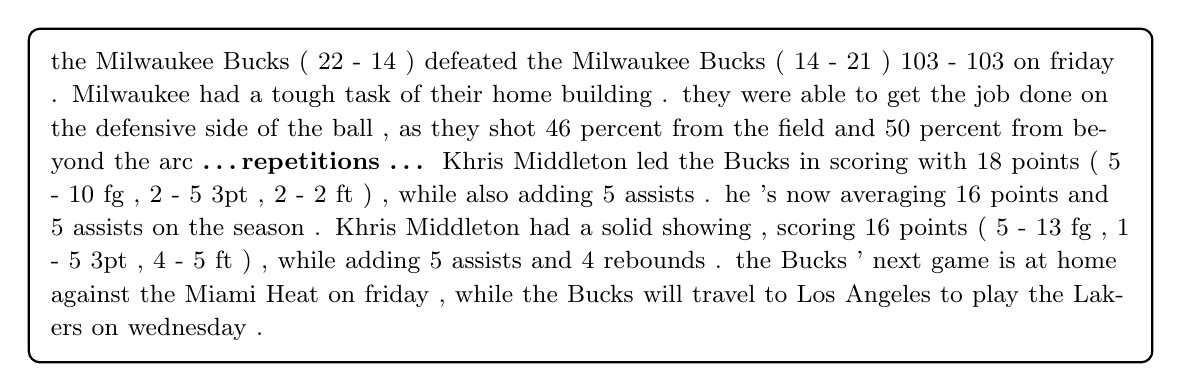
\begin{tikzpicture}
    \node(summary) [rectangle, draw,thick,fill=blue!0,text width=39em, rounded corners, inner sep =8pt, minimum height=1em]{
        \baselineskip=100pt
        \small
        the Milwaukee Bucks ( 22 - 14 ) defeated the Milwaukee Bucks ( 14 - 21 ) 103 - 103 on friday . Milwaukee had a tough task of their home building . they were able to get the job done on the defensive side of the ball , as they shot 46 percent from the field and 50 percent from beyond the arc \textbf{\dots repetitions \dots} Khris Middleton led the Bucks in scoring with 18 points ( 5 - 10 fg , 2 - 5 3pt , 2 - 2 ft ) , while also adding 5 assists . he 's now averaging 16 points and 5 assists on the season . Khris Middleton had a solid showing , scoring 16 points ( 5 - 13 fg , 1 - 5 3pt , 4 - 5 ft ) , while adding 5 assists and 4 rebounds . the Bucks ' next game is at home against the Miami Heat on friday , while the Bucks will travel to Los Angeles to play the Lakers on wednesday .
    };
    \end{tikzpicture} }
    \footnotesize{\textit{Note:} I substitued 4 repetitions of the sentence "the Bucks were able to get the job done on defense , as they shot 46 percent from the field and 50 percent from beyond the arc ." with "\dots repetitions \dots"}
    \caption{\centering An excerpt from a summary generated by the baseline model.} \label{baseline_no_reg_sum}
\end{figure}

\section{Implementation Details}

As stated in the introduction this thesis is highly theoretical and experimental. The implementation serves as proof-of-concept and doesn't aim to be used in the production.

All the models and preprocessing methods were developed in \emph{python 3.8} and \emph{tensorflow 2.4.1}. However the code is compatible with \emph{python 3.6} and \emph{tensorflow 2.3} (the versions used on Artifical Intelligence Cluster (AIC) where the training was executed). The implementation is divided into two modules, \emph{preprocessing} and \emph{training}.

\subsection{Preprocessing Module}

The preprocessing happens in four steps.
\begin{enumerate}
    \item Filtering out the faulty data-points (section \ref{cleaning_section}) from the original dataset.
    \item Extraction and transformation of the summaries from the cleaned dataset.
    \item Byte Pair Encoding of the summaries. (As explained in section \ref{bpeSection} I use the \emph{subword-nmt} module by \citep{sennrich2016}.)
    \item Construction of the dataset from the encoded summaries and the cleaned data. 
\end{enumerate}
Each step is implemented in \emph{python} and the steps are connected by a shell script.

\subsection{Training Module}

The training module contains implementation of layers and models discussed in previous chapters as well as training, evaluation and inference methods. It makes use of \emph{graph execution}\footnote{\url{https://www.tensorflow.org/guide/intro_to_graphs}} during training and \emph{eager execution}\footnote{\url{https://www.tensorflow.org/guide/eager}} during evaluation and prediction.

The code is available at \url{https://github.com/gortibaldik/TTTGen/}.